
\lecture{Normal Approximation of the Binomial}{normal-approximation-to-binomial}
\section{Normal Approximation of the Binomial}

\title{Assessing Normality and the Normal Approximation of the Binomial}
\subtitle{Making the Binomial Distribution Tractable}

%\author{Kelly Black}
%\institute{Clarkson University}
\date{18 February 2015}

\begin{frame}
  \titlepage
\end{frame}

\begin{frame}
  \frametitle{Outline}
  \tableofcontents[hideothersubsections,sectionstyle=show/hide]
\end{frame}

\iftoggle{clicker}{%
  \subsection{Clicker Quiz}


  \begin{frame}
    \frametitle{Clicker Quiz}

    Determine the first quartile (Q1) for the following data: \\
    \begin{tabular}{llllll}
      17 & 16 & 18 & 18 & 13 & 15 
    \end{tabular}
 
    \vfill

    \begin{tabular}{l@{\hspace{3em}}l@{\hspace{3em}}l}
      A:  15 & B: 16 & C: 16.5
    \end{tabular}

    \vfill
    \vfill
    \vfill

  \end{frame}
}




\subsection{Assessing Normality}

\begin{frame}
  \frametitle{Given Data Is It Normally Distributed?}

  Given a set of data you want to know if it is consistent with some
  distribution. \textcolor<1>{red}{\textbf{Here we focus on the normal distribution. }}

  \vfill

  \uncover<2->{%
    The Idea - \textcolor{red}{\textbf{If the random variable is normally distributed then}}
    \begin{itemize}
    \item You can calculate a $z$-statistic for each number in the data
      set.
    \item You can calculate the percentile for each number in the data
      set.
    \item You can calculate a theoretical $z$-statistics for a given
      percentile.  
    \item Plot the actual $z$-statistic vs. the theoretical
      $z$-statistic associated with the data point's percentile.
      \note<2>{The result should be a straight line.}
    \end{itemize}
  }
  
\end{frame}

\begin{frame}
  \frametitle{Normal Probability Plot}

  Given a data set,
  \begin{eqnarray*}
    y_1,~y_2,~y_3,\ldots,y_n,
  \end{eqnarray*}
  \only<1|handout:1>{%
    we construct a normal probability plot to provide an initial
    estimate how closely the data conforms to a normal distribution.
    \vfill
  }

  \only<2-|handout:2->{%
    \begin{enumerate}
      \only<2|handout:2>{%
      \item Sort the data from low to high,
        \begin{eqnarray*}
          x_1,~x_2,~x_3,\ldots,x_n, \\
          x_i & \leq & x_{i+1}.
        \end{eqnarray*}
      }
      \only<2|handout:2>{%
      \item Calculate the sample mean,
        \begin{eqnarray*}
          \bar{x} & = & \frac{x_1+x_2+\cdots+x_n}{n}.
        \end{eqnarray*}
      }
      \only<2|handout:2>{%
      \item Calculate the sample standard deviation,
        \begin{eqnarray*}
          s^2 & = & \frac{(x_1-\bar{x})^2 + (x_2-\bar{x})^2  + \cdots + (x_n-\bar{x})^2}{n-1}, \\
          s & = & \sqrt{s^2}.
        \end{eqnarray*}
      }
      \only<3|handout:3>{%
      \item For each data point compute its percentile within the data
        assuming a normal distribution,
        \begin{eqnarray*}
          f_i & = & \frac{i-\frac{3}{8}}{n+\frac{1}{4}}.
        \end{eqnarray*}
      }
      \only<3|handout:3>{%
      \item Calculate the $z$-statistic associated with $f_i$ by working
        the standard normal table backwards to get $Z^*_i$.
      }
      \only<3|handout:3>{%
      \item Calculate the $z$-statistic associated with $x_i$ using
        \begin{eqnarray*}
          z_i & = & \frac{x_i-\bar{x}}{s}.
        \end{eqnarray*}
      }
      \only<3|handout:3>{%
      \item Plot each data pair, $(z_i,Z^*_i)$, on a plot.
      }
    \end{enumerate}
  }
  
\end{frame}

\begin{frame}
  \frametitle{Example}

  First, nobody does this by hand. {\color{red}This is something that
    is done on a computer.}  \uncover<2->{{\color{blue}You still need to know how
    to interpret these graphs!}}

  \uncover<3->{%
    \begin{columns}

      \column{.4\textwidth}
      Given the data, \\
      \begin{tabular}{llllll}
        17 & 16 & 18 & 18 & 13 & 15
      \end{tabular} \\
      The normal probability plot is shown.

      \column{.5\textwidth}

      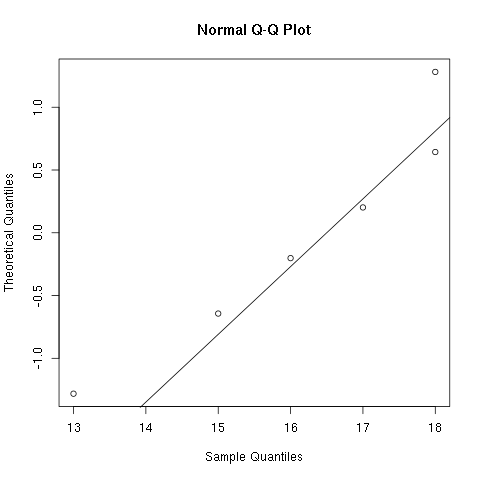
\includegraphics[width=5cm]{img/normalQQEx1}

    \end{columns}
  }
  
  
\end{frame}

\begin{frame}
  \frametitle{Example}


  \begin{columns}

    \column{.4\textwidth}
    Given the data, \\
    \begin{tabular}{llllll}
      9 & 12 & 11 & 8 & 10 & 12
    \end{tabular} \\
    The normal probability plot is shown.

  \column{.5\textwidth}

  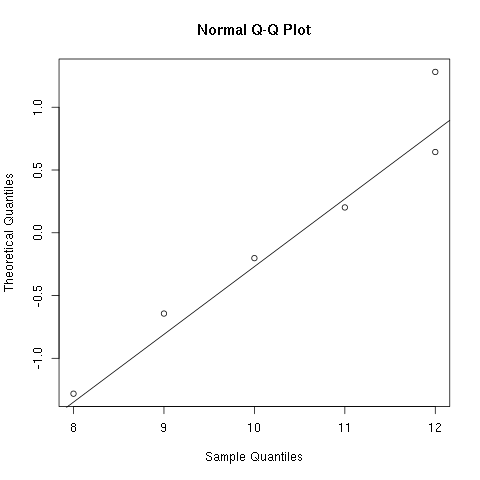
\includegraphics[width=5cm]{img/normalQQEx2}

  \end{columns}
  
  
\end{frame}

\subsection{Binomial Distribution}

\begin{frame}{Normal Distribution, What Is It Good For?}

  The normal distribution is not normally found in practice. There are
  many distributions that are \textbf{\textcolor{red}{close}} to the
  normal distribution.

  \vfill

  For example, in some circumstances, the binomial distribution is
  close enough to the normal distribution that we can use the normal
  distribution instead.

  \vfill
  
\end{frame}


\iftoggle{clicker}{%
  \subsection{Clicker Quiz}


  \begin{frame}
    \frametitle{Clicker Quiz}

    Determine the value of $a$ that satisfies
    \begin{eqnarray*}
      p(z \leq a) & = & 0.95.
    \end{eqnarray*}

    \vfill

    \begin{tabular}{l@{\hspace{3em}}l@{\hspace{3em}}l}
      A: .8289 & B: 1.565 & C: 1.645
    \end{tabular}

    \vfill
    \vfill
    \vfill


  \end{frame}
}




%\subsection{Normal Distribution}
%
%\begin{frame}
%  \frametitle{Example}
%
%  A random variable, $X$, is normally distributed with mean 2.5 and a
%  standard deviation of 3.6. Find $a$ so that
%  \begin{eqnarray*}
%    p(-2.0 \leq X \leq a) & = & 0.80.
%  \end{eqnarray*}
%
%\end{frame}


\begin{frame}{Binomial Distribution}

  Recall the definition of the binomial distribution.

  \vfill

  \begin{definition}[Binomial Distribution]
    \begin{itemize}
    \item There are $N$ experiments.
    \item Each experiment has only two possible outcomes (Yes/No).
    \item Each experiment has a probability $p$ of a ``yes'' outcome.
    \item Each experiment is independent of the others.
    \item We want to know the probability that we obtain $k$ ``yeses.''
    \end{itemize}
    \begin{eqnarray*}
      p(X=k) & = & \prescript{~}{N}{C}_k ~ p^k (1-p)^{N-k}.
    \end{eqnarray*}
  \end{definition}

  \vfill

\end{frame}

\subsection{Binomial Approximation}


\begin{frame}

    Suppose that $X$ is a random variable that follows a binomial
    distribution. It has $N$ repetitions, and the probability of a
    success is $p$. 


  \begin{block}{Binomial Approximation}
    \textbf{IF} $N\cdot p\geq 5$ \textbf{AND} $N\cdot (1-p) \geq 5$
    then $X$ can be approximated using a normal distribution:

    \begin{center}
      \begin{tabular}{ll}
        Mean: & $N\cdot p$, \\
        Std. Dev. & $\sqrt{N\cdot p \cdot (1-p)}$,
      \end{tabular}
    \end{center}

    and

    \begin{eqnarray*}
      p(X \leq a) & \approx &
       p\lp Z \leq \frac{a+0.5-N\cdot p}{\sqrt{N\cdot p \cdot (1-p)}}\rp.
    \end{eqnarray*}

  \end{block}

\end{frame}

\begin{frame}{Binomial Distribution}

  \framezoom<2><3>(0cm,1.0cm)(3cm,3cm)
  \only<1|handout:1>{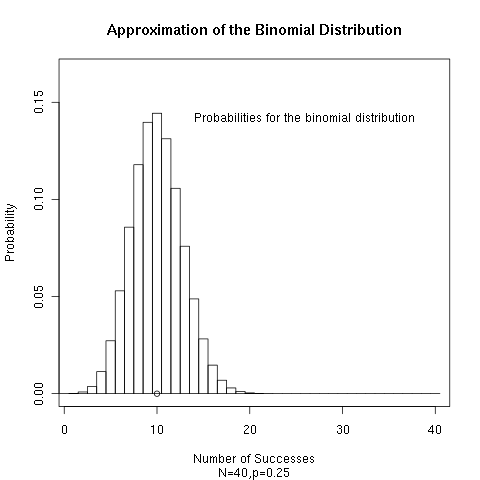
\includegraphics[width=6cm]{img/binomialN40}}
  \only<2-|handout:2>{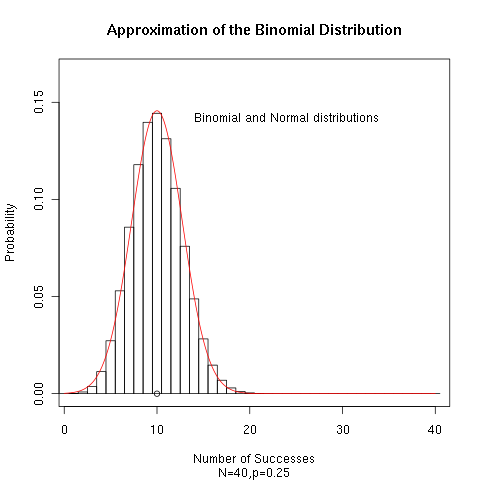
\includegraphics[width=6cm]{img/binomialApproximationN40}}
  
\end{frame}

\subsection{Examples}

\begin{frame}{Example}
  You want to take a poll of eighty employees. You will ask them if
  they like their benefits package. You suspect that 35\% of all
  employees do like their benefits. What is the probability that
  twenty-two or less will say they do?

  \vfill
  \note{You must check that $N\cdot p > 5$ \\}
  \note{You must check that $N\cdot (1-p) > 5$ \\}
  \note{Answer: 0.0985 \\}
\end{frame}


\begin{frame}{Example}
  You want to take a poll of eighty employees. You will ask them if
  they like their benefits package. You suspect that 35\% of all
  employees do like their benefits. Determine the cut-off where there
  is a twenty percent chance that fewer than the cut-off will say
  they do like their benefits.

  \vfill
  \note{You must check that $N\cdot p > 5$ \\}
  \note{You must check that $N\cdot (1-p) > 5$ \\}
  \note{Answer: There is a probability of approximately 20\% that
    fewer than  24 will say that they like their benefits.\\}
\end{frame}


\iftoggle{clicker}{%
  \begin{frame}{Clicker Quiz}
    Clarkson University claims that over eighty percent of all
    students take part in intramural sports. You choose three hundred
    students at random. What is the probability that
    \textcolor{red}{\textbf{more}} than two-hundred and fifty will say
    that they take part in intramural sports?

    \vfill

    \begin{tabular}{l@{\hspace{3em}}l@{\hspace{3em}}l}
      A: 0.0643  & B: 0.4679 & C: 0.9375
    \end{tabular}

    \vfill
    \vfill
    \vfill
    \note{You must check that $N\cdot p > 5$ \\}
    \note{You must check that $N\cdot (1-p) > 5$ \\}

  \end{frame}
}


\begin{frame}{Example}

  The stocks for fifty companies are chosen at random. It is estimated
  that the price of forty-two percent of all stocks will rise. What is
  the probability that twenty five or more of the stocks will rise?

  \vfill
  \vfill

  \note{You must check that $N\cdot p > 5$ \\}
  \note{You must check that $N\cdot (1-p) > 5$ \\}
  \note{Answer: .1587}
  
\end{frame}


% LocalWords:  Clarkson pausesection hideallsubsections
